\documentclass[]{article}

\usepackage[english]{babel}
\usepackage{graphicx}
\usepackage{booktabs}
\usepackage{float}
\usepackage{hyperref}

\title{Some Deep Learning Techniques}
\author{Juan Lao Tebar}

\begin{document}

\maketitle

\begin{abstract}

Deep Convolutional Neural Networks are powerful learning models, specially for image processing. In this practice we classify the CIFAR100 dataset implementing several Deep Learning techniques to improve the learning process and to prevent overfitting, testing different optimizing algorithms, choosing a better activation function, applying dropout, regularizing with weight decay and extending the original dataset with data augmentation.

\end{abstract}

\section{Introduction}

In this practice we analyze the practical effect of several deep learning techniques and methods in a model based on CNN (Convolutional Neural Networks) in order to classify the CIFAR100 dataset.

CIFAR100 is composed by 60,000 32x32 color images labeled over 100 categories. The workflow of this practice consists in defining a baseline model and improving it in the following experiments, step by step.

The code related to this work is public and available at github\footnote{\url{https://github.com/juanlao7/CIFAR100-CNN}}.

\section{Experiments}

We divide the dataset into 40,000 images used for training, 10,000 for validation and 10,000 for testing. On the one hand, we measure the loss of the model by using common cross entropy, while on the other hand we compute its accuracy against training, validation and test data to determine the model's final performance.

\subsection{Baseline}

Our baseline model is composed by three convolutional layers with a kernel size of $3\times3$ and 27, 81, 135 filters respectively; after each convolutional layer we perform a MaxPooling with a pool size of $2\times2$. Finally, this pyramid-schemed stack is connected to two dense layers of 128 units each. We use ReLU as activation function for all the hidden units, and softmax on the output layer. A graphical schema of this model can be seen in figure \ref{f:baseline}.

We train the model in batches of 100 samples using the SGD (Stochastic Gradient Descent) optimizer with a learning rate of 0.001, no momentum and no learning rate decay. Our stop criteria consists in detecting a minimum in the validation loss, stopping the training 15 epochs after it is reached.

Table \ref{t:baseline} shows the results obtained with this model, using the script \texttt{baseline.py}.

\begin{table}[H]
	\centering
	\label{t:baseline}
	\begin{tabular}{@{}cccccc@{}}
		\toprule
		\multicolumn{2}{c}{Training} & \multicolumn{2}{c}{Validation} & \multicolumn{2}{c}{Test} \\ \midrule
		Loss         & Accuracy      & Loss          & Accuracy       & Loss       & Accuracy    \\
		\midrule
		1.8287       & 0.5116        & 2.7988        & 0.3407         & 2.7651     & 0.3500      \\ \bottomrule
	\end{tabular}
	\caption{Results of the baseline model.}
\end{table}

\subsection{Activation Function}

Clevert, Unterthiner, \& Hochreiter, 2016 \cite{clevert2015fast} found that using ELU instead of ReLU not only speeds up the learning process in deep neural networks, but also leads to higher classification accuracies: ``In contrast to ReLUs, ELUs have negative values which allows them to push mean unit activations closer to zero like batch normalization but with lower computational complexity. Mean shifts toward zero speed up learning by bringing the normal gradient closer to the unit natural gradient because of a reduced bias shift effect''.

Clevert et al., 2016 test their hypothesis also on CIFAR100, the same dataset we use in this practice. In this experiment we aim to reproduce similar results, testing different activation functions---ReLU, ELU and softplus---for the hidden layers of our model.

Table \ref{t:act} shows the results obtained with each activation function, using the script \texttt{activation.py}, while figure \ref{f:act1} shows the evolution of the loss during the training.

\begin{table}[H]
	\centering
	\label{t:act}
	\begin{tabular}{@{}ccccccc@{}}
		\toprule
		& \multicolumn{2}{c}{Training} & \multicolumn{2}{c}{Validation} & \multicolumn{2}{c}{Test} \\ \midrule
		& Loss         & Accuracy      & Loss          & Accuracy       & Loss       & Accuracy    \\
		\midrule
		ReLU     & 1.8287       & 0.5116        & 2.7988        & 0.3407         & 2.7651     & 0.3500      \\
		ELU      & 1.6771       & 0.5518        & 2.6451        & 0.3706         & 2.5976     & 0.3782      \\
		Softplus & 2.1089       & 0.4520        & 3.0834        & 0.2915         & 3.0400     & 0.3033      \\ \bottomrule
	\end{tabular}
	\caption{Results after testing different activation functions.}
\end{table}

\begin{figure}[H]
	\centering
	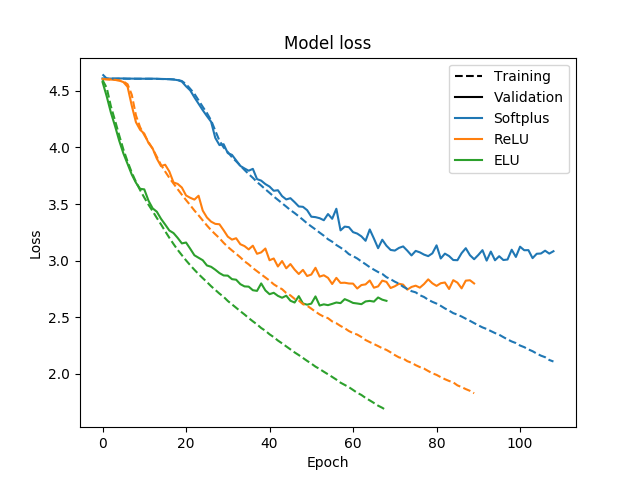
\includegraphics[width=0.5\textwidth]{activation_loss}
	\caption{Validation and training loss with each activation function.}
	\label{f:act1}
\end{figure}

As we can see in figure \ref{f:act1}, validation loss on ELUs take a lesser number of epochs to converge, and the convergence value is lower than the one obtained with ReLUs or softplus, confirming the results obtained by Clevert et al., 2016.

In the following experiments we establish ELU as the activation function for all the units of the hidden layers.

\subsection{Optimizer}

In comparison with the classic SGD, adaptive optimizing algorithms may improve the accuracy of our model. In this experiment we test the following ones:

\begin{itemize}
	\item RMSprop \cite{tieleman2012lecture} with a learning rate of 0.001, $ \rho = 0.9 $, $ \varepsilon = 1 \cdot 10^{-8} $ and no learning rate decay.
	\item Adagrad \cite{duchi2011adaptive} with a learning rate of 0.01, $ \varepsilon = 1 \cdot 10^{-8} $ and no learning rate decay.
	\item Adadelta \cite{zeiler2012adadelta} with a learning rate of 1.0, $ \rho = 0.95 $, $ \varepsilon = 1 \cdot 10^{-8} $ and no learning rate decay.
	\item Adam \cite{kingma2014adam} with a learning rate of 0.001, $ \beta_1 = 0.9 $, $ \beta_2 = 0.999 $, $ \varepsilon = 1 \cdot 10^{-8} $ and no learning rate decay.
	\item Adamax \cite{kingma2014adam} with a learning rate of 0.002, $ \beta_1 = 0.9 $, $ \beta_2 = 0.999 $, $ \varepsilon = 1 \cdot 10^{-8} $ and no learning rate decay.
	\item Nadam \cite{dozat2016incorporating} with a learning rate of 0.002, $ \beta_1 = 0.9 $, $ \beta_2 = 0.999 $, $ \varepsilon = 1 \cdot 10^{-8} $ and a schedule decay of 0.004.
\end{itemize}

The hyperparameters of each optimizer take as value the default proposed by keras framework\footnote{\url{https://keras.io/optimizers/}}.

Table \ref{t:opt} shows the results obtained with each optimizer, using the script \texttt{optimizer.py}, while figure \ref{f:opt1} shows the evolution of the loss during the training.

\begin{table}[H]
	\centering
	\label{t:opt}
	\begin{tabular}{@{}ccccccc@{}}
		\toprule
		& \multicolumn{2}{c}{Training} & \multicolumn{2}{c}{Validation} & \multicolumn{2}{c}{Test} \\ \midrule
		& Loss         & Accuracy      & Loss          & Accuracy       & Loss       & Accuracy    \\
		\midrule
		SGD      & 1.5802       & 0.5718        & 2.6983        & 0.3671         & 2.6934     & 0.3672      \\
		RMSprop  & 0.6178       & 0.8073        & 4.1684        & 0.3504         & 4.1685     & 0.3573      \\
		Adagrad  & 1.5254       & 0.5882        & 2.5027        & 0.3970         & 2.4637     & 0.4096      \\
		Adadelta & 1.0975       & 0.6920        & 3.0320        & 0.3793         & 2.9825     & 0.3795      \\
		Adam     & 0.4316       & 0.8635        & 4.5640        & 0.3567         & 4.5586     & 0.3608      \\
		Adamax   & 0.6595       & 0.8019        & 3.7275        & 0.3652         & 3.7116     & 0.3696      \\
		Nadam    & 0.4711       & 0.8477        & 5.3245        & 0.3281         & 5.2915     & 0.3366      \\ \bottomrule
	\end{tabular}
	\caption{Results obtained with each optimizer.}
\end{table}

\begin{figure}[H]
	\centering
	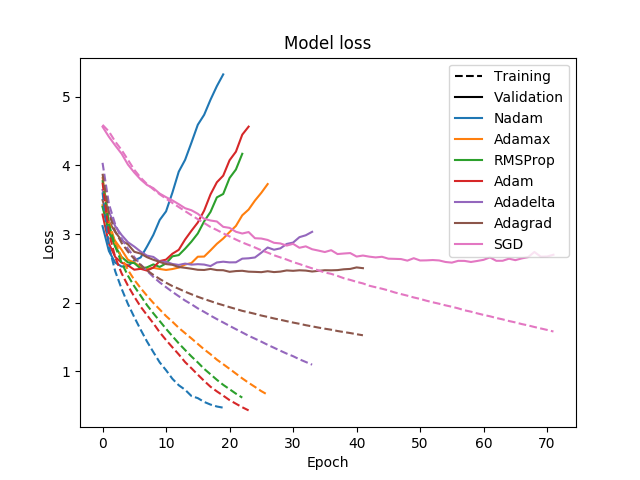
\includegraphics[width=0.5\textwidth]{optimizer_loss}
	\caption{Validation and training loss with each optimizer.}
	\label{f:opt1}
\end{figure}

As we see in figure \ref{f:opt1}, Nadam training curve is the most pronounced, indicating that it is a powerful learning algorithm, despite it obtains the worst validation loss at the end of the process due to overfitting. On the other hand Adagrad has the best validation loss, but with a much flatter training curve.

In the following experiments we try different regularization methods on Adagrad and Nadam.

\subsection{Dropout}

Dropout is considered a simple and powerful regularization method. \cite{srivastava2014dropout} ``The key idea is to randomly drop units (along with their connections) from the neural network during training. This prevents units from co-adapting too much. During training, dropout samples from an exponential number of different ``thinned'' networks. At test time, it is easy to approximate the effect of averaging the predictions of all these thinned networks by simply using a single unthinned network that has smaller weights. This significantly reduces overfitting and gives major improvements over other regularization methods''.

In this experiment we apply different dropout values---25\%, 50\% and 75\%---after each MaxPooling layer of the model and between the final hidden dense layers, as shown in figure \ref{f:drop1}.

Table \ref{t:drop} shows the results obtained with each dropout value, using the script \texttt{dropout.py}, while figures \ref{f:drop2} and \ref{f:drop3} show the evolution of the loss during the training for Adagrad and Nadam respectively.

\begin{table}[H]
	\centering
	\label{t:drop}
	\begin{tabular}{@{}cccccccc@{}}
		\toprule
		&      & \multicolumn{2}{c}{Training} & \multicolumn{2}{c}{Validation} & \multicolumn{2}{c}{Test} \\ \midrule
		&      & Loss         & Accuracy      & Loss          & Accuracy       & Loss       & Accuracy    \\
		\midrule
		Adagrad & 0\%  & 1.5133       & 0.5914        & 2.5515        & 0.3888         & 2.5019     & 0.3986      \\
		& 25\% & 2.0568       & 0.4801        & 2.2222        & 0.4237         & 2.1943     & 0.4290      \\
		& 50\% & 2.9340       & 0.2691        & 3.2668        & 0.2193         & 3.2500     & 0.2238      \\
		& 75\% & 3.7911       & 0.1110        & 4.6237        & 0.0455         & 4.6116     & 0.0449      \\
		\midrule
		Nadam   & 0\%  & 0.4454       & 0.8542        & 5.2706        & 0.3244         & 5.2349     & 0.3358      \\
		& 25\% & 2.0185       & 0.4572        & 2.2736        & 0.4279         & 2.2447     & 0.4349      \\
		& 50\% & 3.0121       & 0.2495        & 3.0368        & 0.2564         & 2.9962     & 0.2608      \\
		& 75\% & 3.9112       & 0.0885        & 5.0259        & 0.0281         & 5.0184     & 0.0286      \\ \bottomrule
	\end{tabular}
	\caption{Results obtained with each dropout value.}
\end{table}

\begin{figure}[H]
	\centering
	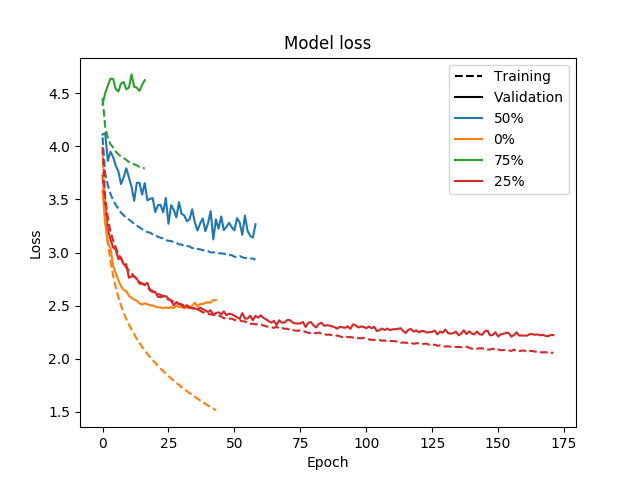
\includegraphics[width=0.5\textwidth]{dropout_adagrad_loss}
	\caption{Validation and training loss with each dropout factor, with Adagrad optimizer.}
	\label{f:drop2}
\end{figure}

\begin{figure}[H]
	\centering
	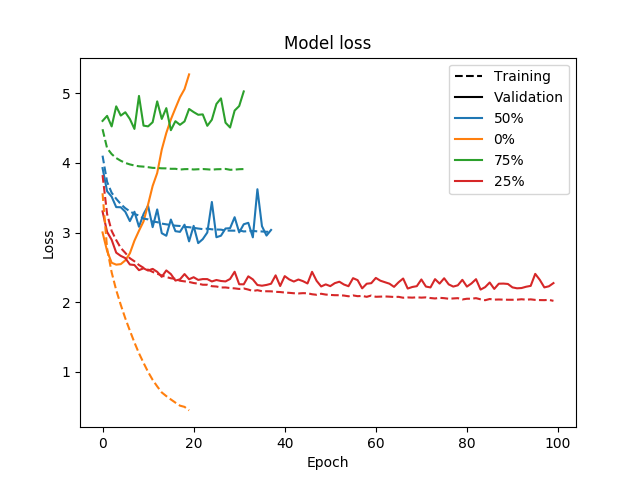
\includegraphics[width=0.5\textwidth]{dropout_nadam_loss}
	\caption{Validation and training loss with each dropout factor, with Nadam optimizer.}
	\label{f:drop3}
\end{figure}

As we can see in figures \ref{f:drop2} and \ref{f:drop3}, a dropout of 25\% successfully regularizes the network, decreasing the gap between validation and training losses; as a result, the resulting validation accuracy is higher than the one obtained with unregularized models, no matter the optimizing algorithm. Higher dropout factors obtain worse results than our original approach.

Without applying regularization, Adagrad gets a better accuracy than Nadam; however, after applying dropout, Nadam gets a better mark.

In the following experiments we always apply a dropout factor of 25\%.

\subsection{Weight Decay}

Another common regularization method consists in applying a weight decay factor to the unit weights during the training. \cite{krogh1992simple} ``It is proven that a weight decay has two effects in a linear network. First, it suppresses any irrelevant components of the weight vector by choosing the smallest vector that solves the learning problem. Second, if the size is chosen right, a weight decay can suppress some of the effects of static noise on the targets, which improves generalization quite a lot''.

In the first part of this experiment we regularize the weights of the kernel of each convolutional layer and the weights of our two dense layers using L1, L2 and L1+L2, with a factor of 0.0001.

Table \ref{t:ker1} shows the results obtained with each decay function, using the script \texttt{weight1.py}, while figures \ref{f:ker1} and \ref{f:ker2} show the evolution of the loss and accuracy during the training for Adagrad and figures \ref{f:ker3} and \ref{f:ker4} show the same evolution but for Nadam.

\begin{table}[H]
	\centering
	\label{t:ker1}
	\begin{tabular}{@{}cccccccc@{}}
		\toprule
		&       & \multicolumn{2}{c}{Training} & \multicolumn{2}{c}{Validation} & \multicolumn{2}{c}{Test} \\ \midrule
		&       & Loss         & Accuracy      & Loss          & Accuracy       & Loss       & Accuracy    \\
		\midrule
		Adagrad & None  & 1.9783       & 0.4666        & 2.1632        & 0.4385         & 2.1409     & 0.4454      \\
		& L1    & 2.6520       & 0.4173        & 2.6633        & 0.4233         & 2.6385     & 0.4280      \\
		& L2    & 2.0478       & 0.4721        & 2.2159        & 0.4503         & 2.1998     & 0.4519      \\
		& L1+L2 & 4.0246       & 0.1105        & 4.0332        & 0.1102         & 4.0171     & 0.1116      \\
		\midrule
		Nadam   & None  & 2.0566       & 0.4439        & 2.2329        & 0.4359         & 2.1925     & 0.4390      \\
		& L1    & 2.9900       & 0.3711        & 2.9063        & 0.3956         & 2.8995     & 0.4009      \\
		& L2    & 2.2500       & 0.4552        & 2.4368        & 0.4326         & 2.3947     & 0.4375      \\
		& L1+L2 & 3.8634       & 0.1807        & 3.8171        & 0.2031         & 3.7988     & 0.2064      \\ \bottomrule
	\end{tabular}
	\caption{Results obtained with each decay function.}
\end{table}

\begin{figure}[H]
	\centering
	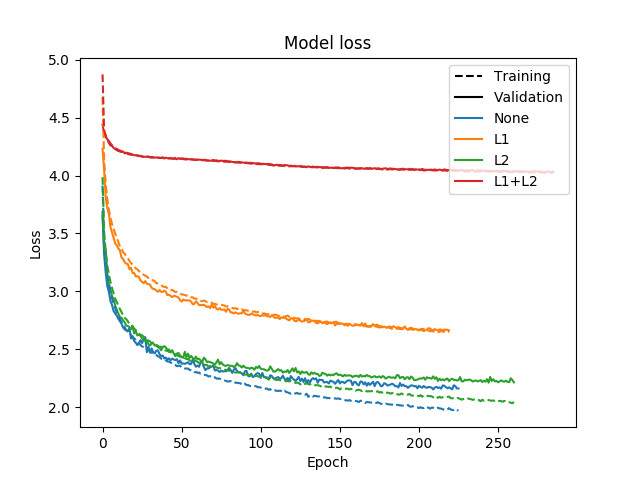
\includegraphics[width=0.5\textwidth]{weight1_adagrad_loss}
	\caption{Validation and training loss with each weight decay function, with Adagrad optimizer.}
	\label{f:ker1}
\end{figure}

\begin{figure}[H]
	\centering
	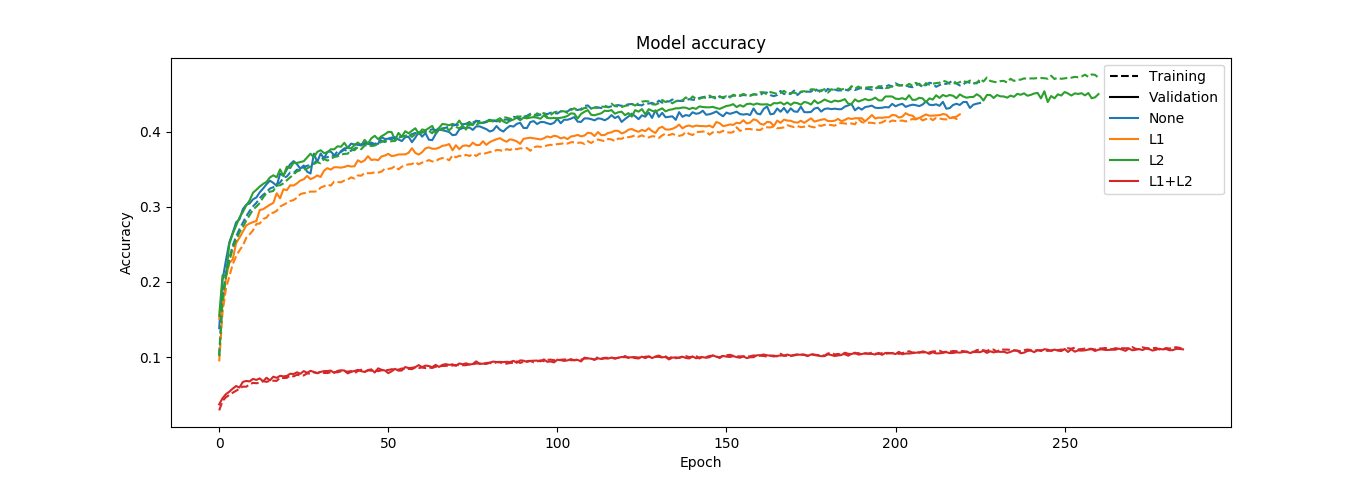
\includegraphics[width=\textwidth]{weight1_adagrad_acc}
	\caption{Validation and training accuracy with each weight decay function, with Adagrad optimizer.}
	\label{f:ker2}
\end{figure}

\begin{figure}[H]
	\centering
	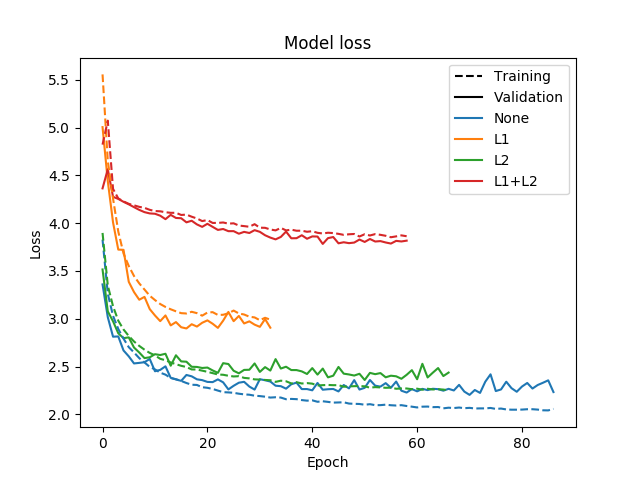
\includegraphics[width=0.5\textwidth]{weight1_nadam_loss}
	\caption{Validation and training loss with each weight decay function, with Nadam optimizer.}
	\label{f:ker3}
\end{figure}

\begin{figure}[H]
	\centering
	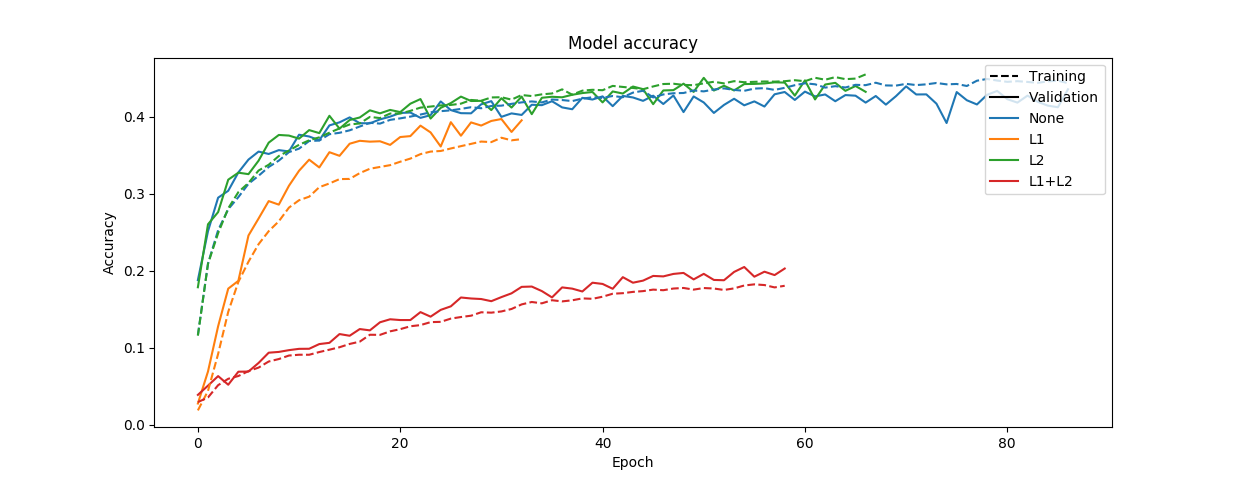
\includegraphics[width=\textwidth]{weight1_nadam_acc}
	\caption{Validation and training accuracy with each weight decay function, with Nadam optimizer.}
	\label{f:ker4}
\end{figure}

In the second part of this experiment we test different weight decay factors---0.01, 0.001, 0.0001 and 0.00001---on L2, the function that gets the best results in the previous experiment. Table \ref{t:ker2} shows the results obtained with different weight decay factors, using the script \texttt{weight2.py}, while figures \ref{f:ker5} and \ref{f:ker6} show the evolution of the loss during the training for Adagrad and figures \ref{f:ker7} and \ref{f:ker8} show the same evolution but for Nadam.

\begin{table}[H]
	\centering
	\label{t:ker2}
	\begin{tabular}{@{}cccccccc@{}}
		\toprule
		&         & \multicolumn{2}{c}{Training} & \multicolumn{2}{c}{Validation} & \multicolumn{2}{c}{Test} \\ \midrule
		&         & Loss         & Accuracy      & Loss          & Accuracy       & Loss       & Accuracy    \\
		\midrule
		Adagrad & 0.00000 & 1.9315       & 0.4768        & 2.1750        & 0.4384         & 2.1495     & 0.4467      \\
		& 0.00001 & 2.0028       & 0.4649        & 2.1890        & 0.4381         & 2.1668     & 0.4436      \\
		& 0.00010 & 2.0476       & 0.4744        & 2.2444        & 0.4453         & 2.2170     & 0.4500      \\
		& 0.00100 & 2.4145       & 0.4508        & 2.4900        & 0.4452         & 2.4717     & 0.4465      \\
		& 0.01000 & 3.5690       & 0.2304        & 3.5481        & 0.2379         & 3.5214     & 0.2477      \\
		\midrule
		Nadam   & 0.00000 & 2.0566       & 0.4439        & 2.2329        & 0.4359         & 2.1925     & 0.4390      \\
		& 0.00001 & 2.1221       & 0.4444        & 2.4286        & 0.4064         & 2.3950     & 0.4120      \\
		& 0.00010 & 2.2500       & 0.4552        & 2.4368        & 0.4326         & 2.3947     & 0.4375      \\
		& 0.00100 & 2.7790       & 0.4075        & 2.7620        & 0.4197         & 2.7442     & 0.4227      \\
		& 0.01000 & 3.7726       & 0.2138        & 3.7417        & 0.2169         & 3.7167     & 0.2224      \\ \bottomrule
	\end{tabular}
	\caption{Results obtained with each weight decay factor.}
\end{table}

\begin{figure}[H]
	\centering
	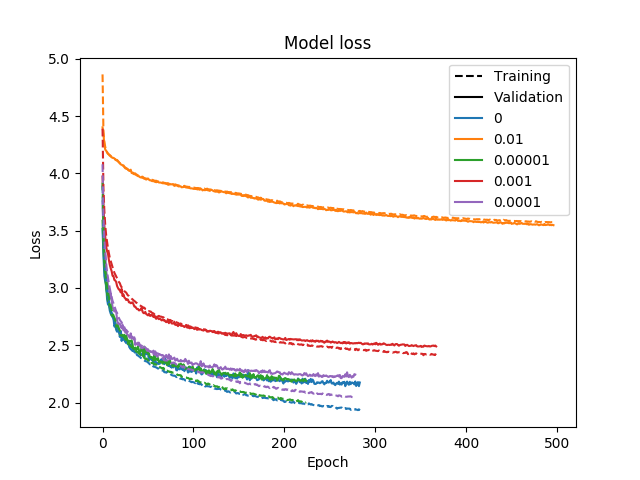
\includegraphics[width=0.5\textwidth]{weight2_adagrad_loss}
	\caption{Validation and training loss with each weight decay factor, with Adagrad optimizer.}
	\label{f:ker5}
\end{figure}

\begin{figure}[H]
	\centering
	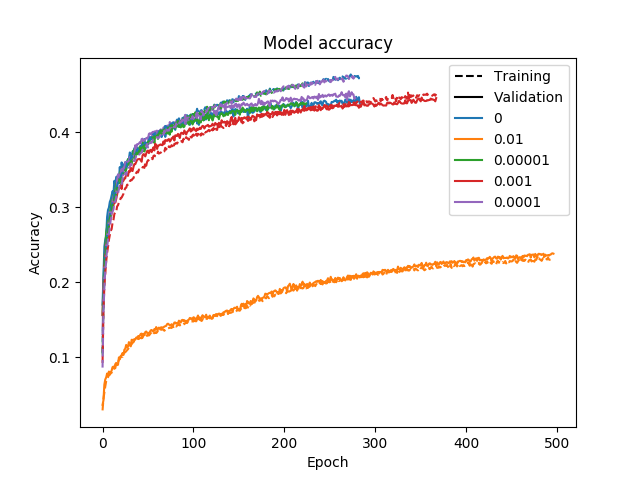
\includegraphics[width=0.5\textwidth]{weight2_adagrad_acc}
	\caption{Validation and training accuracy with each weight decay factor, with Adagrad optimizer.}
	\label{f:ker6}
\end{figure}

\begin{figure}[H]
	\centering
	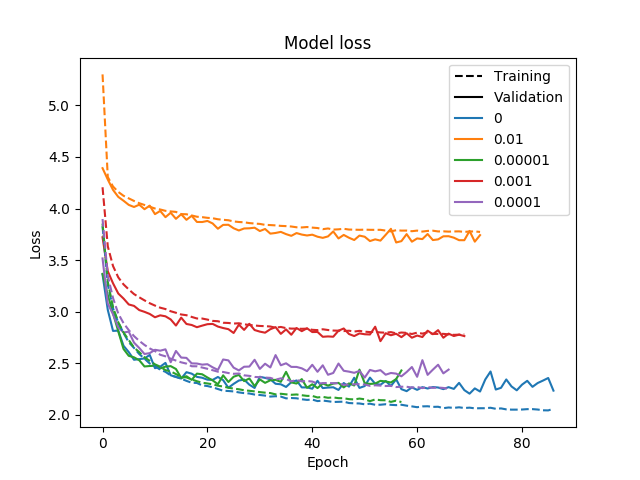
\includegraphics[width=0.5\textwidth]{weight2_nadam_loss}
	\caption{Validation and training loss with each weight decay factor, with Nadam optimizer.}
	\label{f:ker7}
\end{figure}

\begin{figure}[H]
	\centering
	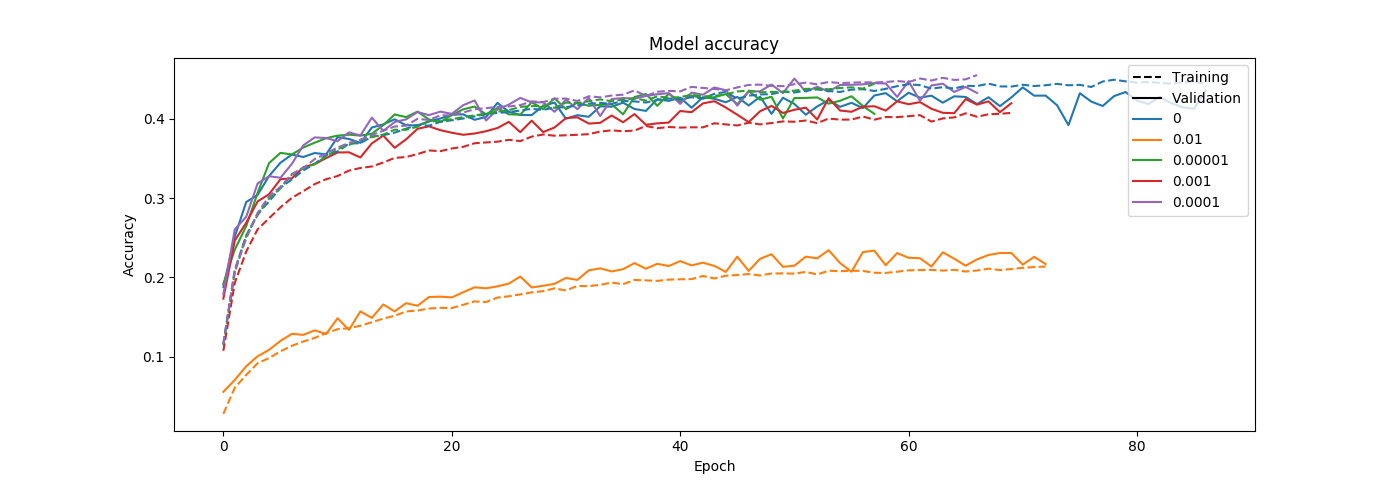
\includegraphics[width=\textwidth]{weight2_nadam_acc}
	\caption{Validation and training accuracy with each weight decay factor, with Nadam optimizer.}
	\label{f:ker8}
\end{figure}

As we can see, we obtain the lowest loss we do not apply weight decay, no matter the optimizer. However, we obtain a slightly better accuracy in Adagrad with an L2 weight decay of 0.0001. With this configuration Adagrad performs better than Nadam, obtaining the best test accuracy we have achieved until now.

From now on, we test only Adagrad with L2 weight decay of 0.0001.

\subsection{Data Augmentation}

An easy way of improving generalization and reduce overfitting when working with images consists in training the model with an infinite number of new samples generated through slightly random modifications of the original dataset.

In this experiment we test the effect of performing random changes in our input:

\begin{itemize}
	\item Rotation of 15 degrees.
	\item Width shift of 10%.
	\item Height shift of 10%.
	\item Shear transformation of 10%.
	\item Zoom of 20%.
	\item Horizontal flip.
\end{itemize}

Table \ref{t:data1} shows the results obtained with each modification, using the script \texttt{data\_augmentation.py}, while figure \ref{f:data1} shows the evolution of the loss during the training.

\begin{table}[H]
	\centering
	\label{t:data1}
	\begin{tabular}{@{}ccccccc@{}}
		\toprule
		& \multicolumn{2}{c}{Training} & \multicolumn{2}{c}{Validation} & \multicolumn{2}{c}{Test} \\ \midrule
		& Loss         & Accuracy      & Loss          & Accuracy       & Loss       & Accuracy    \\
		\midrule
		No augmentation   & 2.0969       & 0.4636        & 2.2752        & 0.4428         & 2.2363     & 0.4485      \\
		Rotation 15 deg.  & 2.4999       & 0.3734        & 2.5400        & 0.3775         & 2.4199     & 0.3952      \\
		Width shift 10\%  & 2.2479       & 0.4298        & 2.2945        & 0.4322         & 2.2131     & 0.4466      \\
		Height shift 10\% & 2.2337       & 0.4306        & 2.3807        & 0.4162         & 2.2925     & 0.4283      \\
		Shear 10\%        & 2.2063       & 0.4317        & 2.4211        & 0.3997         & 2.4163     & 0.4054      \\
		Zoom 20\%         & 2.3279       & 0.4087        & 2.4591        & 0.4006         & 2.3460     & 0.4203      \\
		Horizontal flip   & 2.3008       & 0.4143        & 2.3935        & 0.4036         & 2.3971     & 0.4061      \\ \bottomrule
	\end{tabular}
	\caption{Results obtained with each modification.}
\end{table}

\begin{figure}[H]
	\centering
	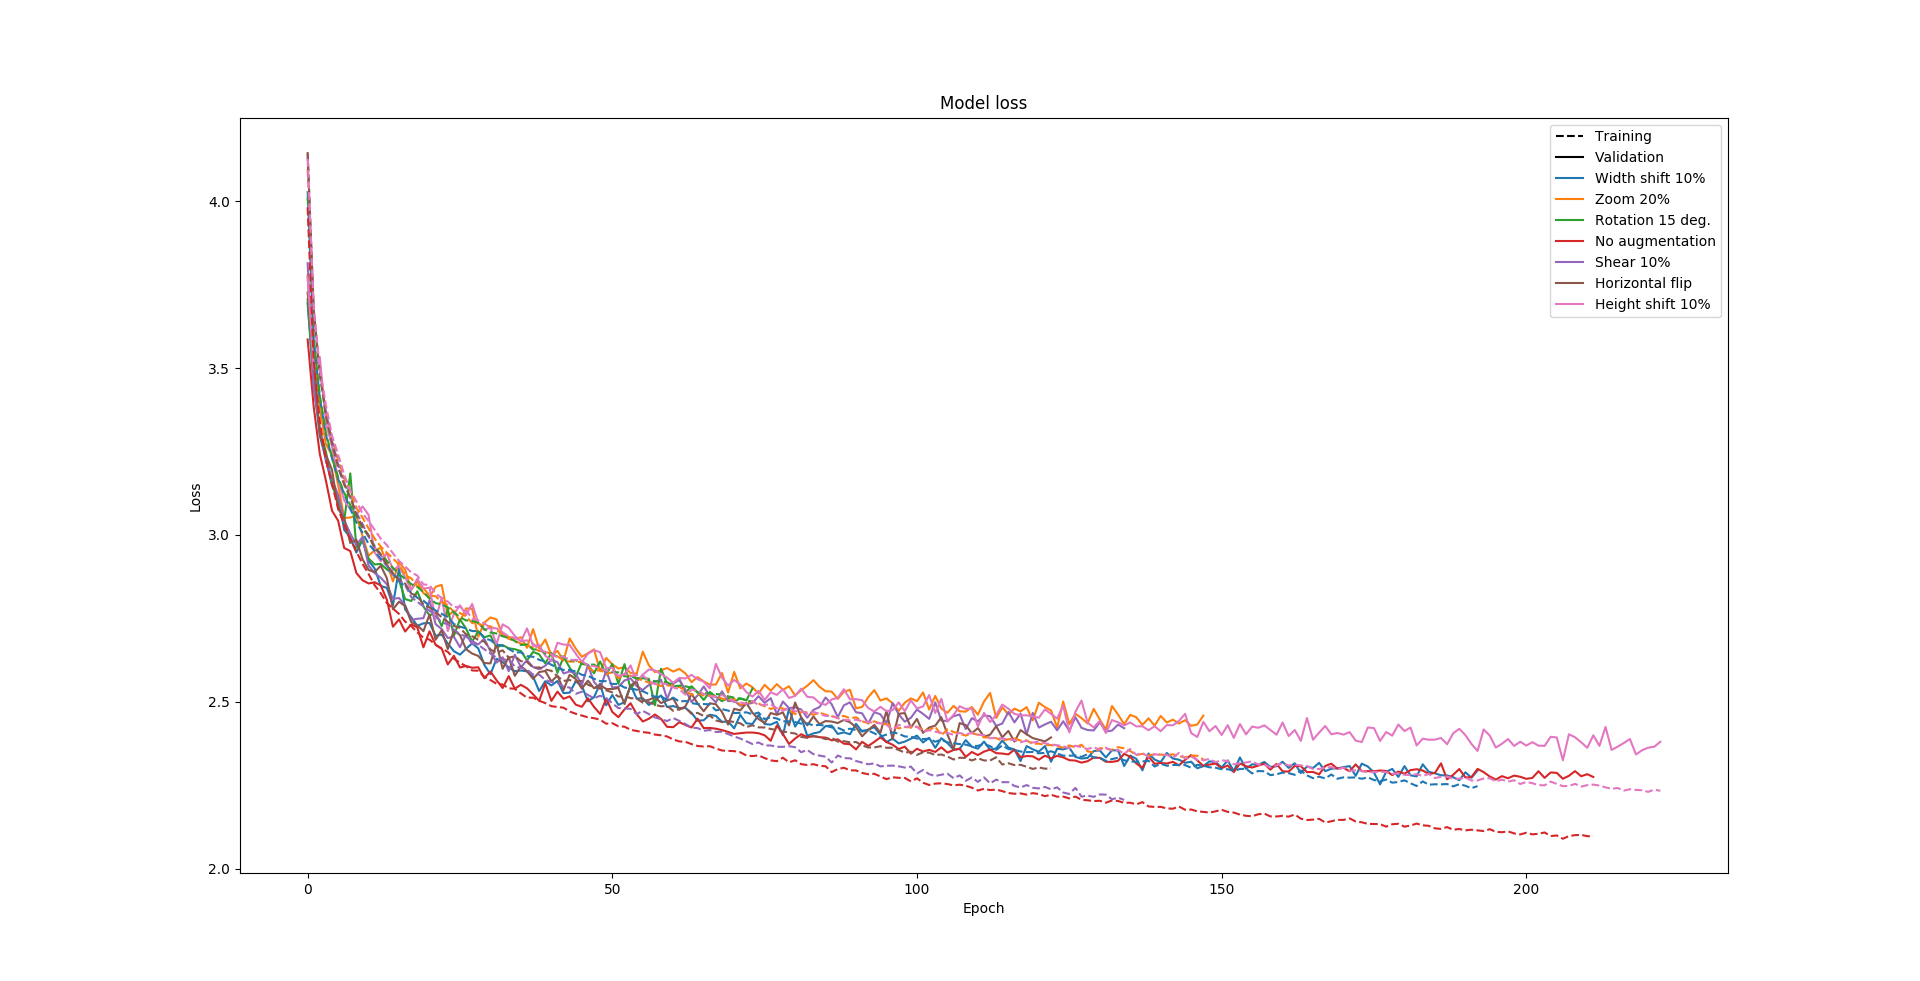
\includegraphics[width=\textwidth]{data_augmentation_loss}
	\caption{Validation and training loss with each modification.}
	\label{f:data1}
\end{figure}

As we can see, data augmentation does not improve the test accuracy of the model, and in some cases it makes it even worse.

\subsection{An Additional Experiment}

Since we applied dropout and weight decay, our model does not overfit anymore, so data augmentation does not improve the result.

In order to have a better idea about the effect of data augmentation in unregularized models, in this experiment we test the performance of RMSprop with data augmentation, without applying dropout or weight decay.

Table \ref{t:rms1} shows the results obtained with each modification, using the script \texttt{data\_augmentation.py}, while figure \ref{f:rms1} shows the evolution of the loss during the training.

\begin{table}[H]
	\centering
	\label{t:rms1}
	\begin{tabular}{@{}ccccccc@{}}
		\toprule
		& \multicolumn{2}{c}{Training} & \multicolumn{2}{c}{Validation} & \multicolumn{2}{c}{Test} \\ \midrule
		& Loss         & Accuracy      & Loss          & Accuracy       & Loss       & Accuracy    \\
		\midrule
		No augmentation   & 0.4384       & 0.8646        & 5.0818        & 0.2979         & 4.9563     & 0.3061      \\
		Rotation 15 deg.  & 1.1264       & 0.6706        & 3.6748        & 0.3125         & 3.4489     & 0.3419      \\
		Width shift 10\%  & 1.2182       & 0.6452        & 2.7489        & 4.4089         & 2.6997     & 0.4120      \\
		Height shift 10\% & 1.1220       & 0.6775        & 3.5430        & 0.3175         & 3.4832     & 0.3328      \\
		Shear 10\%        & 0.5842       & 0.8157        & 4.4306        & 0.3362         & 4.4646     & 0.3266      \\
		Zoom 20\%         & 1.2352       & 0.6422        & 2.9879        & 0.3730         & 2.8393     & 0.3971      \\
		Horizontal flip   & 1.0532       & 0.6994        & 3.7813        & 0.3016         & 3.6553     & 0.3076      \\ \bottomrule
	\end{tabular}
	\caption{Results obtained with each modification on RMSprop.}
\end{table}

\begin{figure}[H]
	\centering
	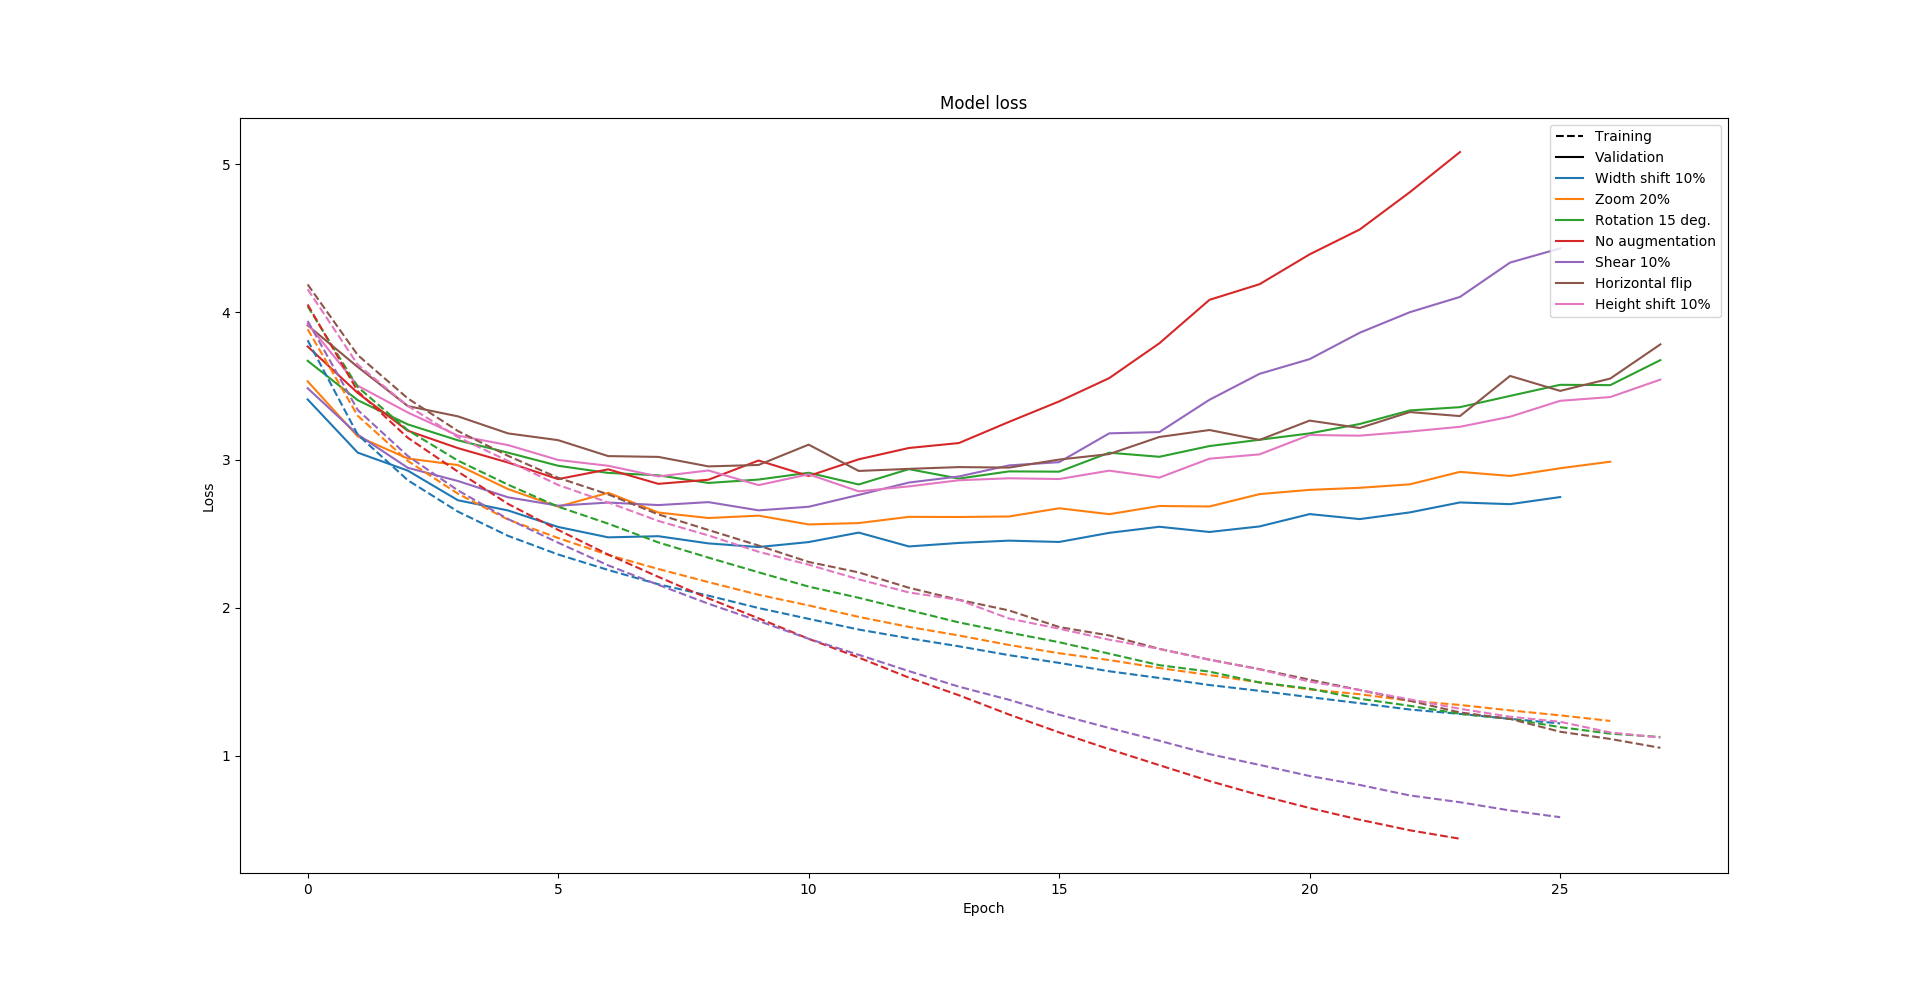
\includegraphics[width=\textwidth]{last1_loss}
	\caption{Validation and training loss with each modification on RMSprop.}
	\label{f:rms1}
\end{figure}

As we can see, in this case, data augmentation prevents overfitting. In the next experiment we apply all the modifications at the same time.

Table \ref{t:rms2} shows the results obtained in each case, using the script \texttt{data\_augmentation.py}, while figure \ref{f:rms2} shows the evolution of the loss during the training.

\begin{table}[H]
	\centering
	\label{t:rms2}
	\begin{tabular}{@{}ccccccc@{}}
		\toprule
		& \multicolumn{2}{c}{Training} & \multicolumn{2}{c}{Validation} & \multicolumn{2}{c}{Test} \\ \midrule
		& Loss         & Accuracy      & Loss          & Accuracy       & Loss       & Accuracy    \\
		\midrule
		No augmentation & 0.4384       & 0.8646        & 5.0818        & 0.2979         & 4.9563     & 0.3061      \\
		Augmented       & 1.7239       & 0.5301        & 2.2968        & 0.4311         & 1.9836     & 0.4941      \\ \bottomrule
	\end{tabular}
	\caption{Results obtained with all modifications on RMSprop.}
\end{table}

\begin{figure}[H]
	\centering
	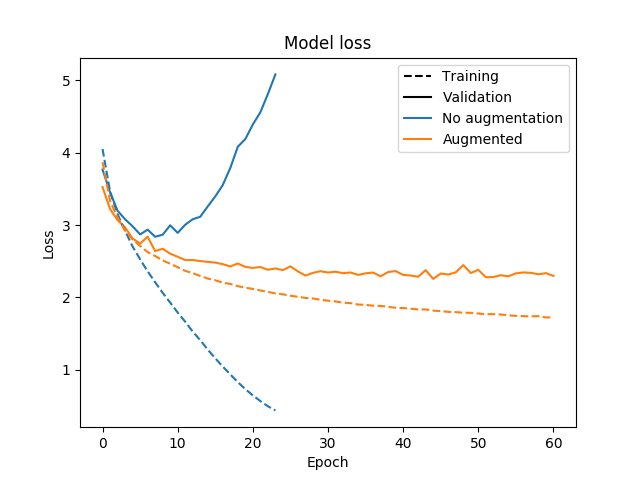
\includegraphics[width=0.5\textwidth]{last2_loss}
	\caption{Validation and training loss with all modifications on RMSprop.}
	\label{f:rms2}
\end{figure}

As we can see, now the model does not overfit the training data, and even obtains the best test accuracy we have achieved until now.

\section{Discussion}

In this work we have seen how the activation function plays an important role in the learning process, and we have discovered that ELU leads to a considerable improvement compared to the common ReLU or to other continuous functions such as softplus. The reason behind this, as stated by Clevert et al., 2016: ``ELUs have negative values which allows them to push mean unit activations closer to zero like batch normalization but with lower computational complexity. Mean shifts toward zero speed up learning by bringing the normal gradient closer to the unit natural gradient because of a reduced bias shift effect''.

Regarding to the optimizer, we have seen that a lot of adaptive algorithms overfit the training data, specially Nadam and RMSprop.

We have found that a dropout of 25\% is enough to avoid overfitting, since it ``prevents units from co-adapting too much''. \cite{srivastava2014dropout} In addition to this, an L2 weight decay of 0.0001 applies an additional regularization that gives slightly better results.

Regarding to data augmentation, our regularized model has not shown any improvement, because it does not overfit the training data anymore. However, when we have tried an unregularized model trained with a strong optimizer---RMSprop---, we have observed a huge improvement in the validation and test accuracies.

\section{Conclusions and Future Work}

In this practice we have tested several deep learning techniques in order to obtain a good model for classifying CIFAR100. We have observed that the general process consists in two parts: making a powerful learning model and, after obtaining it, applying regularization to improve generalization.

When we check out the general validation loss evolution of the latest experiments, we can see that the learning process stops too early. In the future we could test higher validation patience levels and it may lead to better results. In addition, we must note that staying with the model that offers the minimum validation loss---instead of staying with the model of the last epoch---would also give better test accuracies, of course.

With regard to regularization, it would be interesting to try the effect of different batch sizes, as well as refining the optimizer hyperparameters.

Finally, different network topologies may lead to better results too. In this practice we have tested a simple CNN model of three convolutional layers and two dense layers, but a more complex model, or even a recursive one---such as attention models \cite{itti1998model}---may give better results.

\bibliography{bibfile}{}
\bibliographystyle{plain}

\pagebreak

\appendix

\section{Network Structures}

\begin{figure}[H]
	\centering
	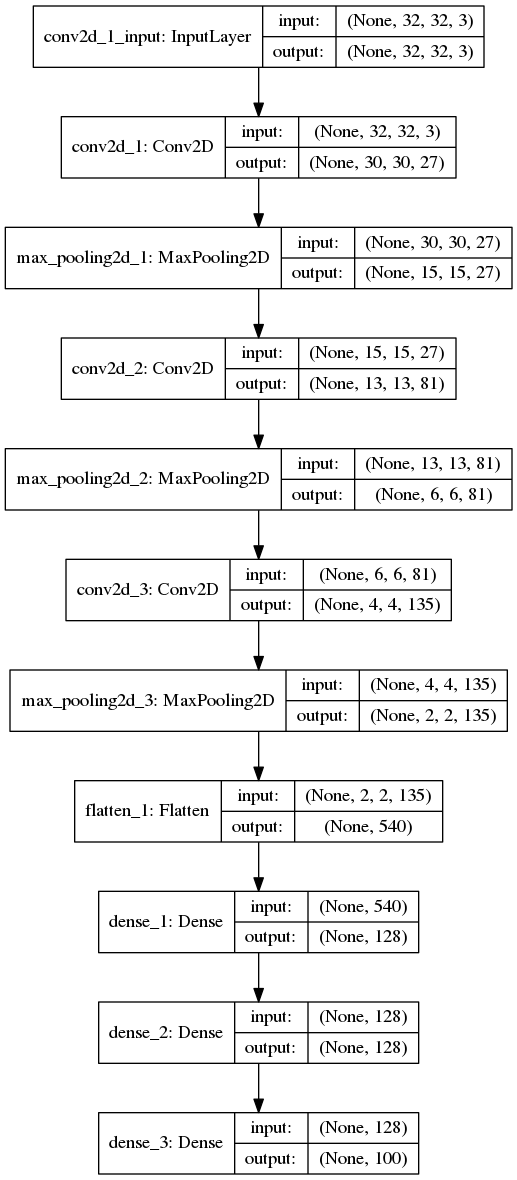
\includegraphics[width=0.5\textwidth]{baseline}
	\caption{Structure of the CNN model.}
	\label{f:baseline}
\end{figure}

\begin{figure}[H]
	\centering
	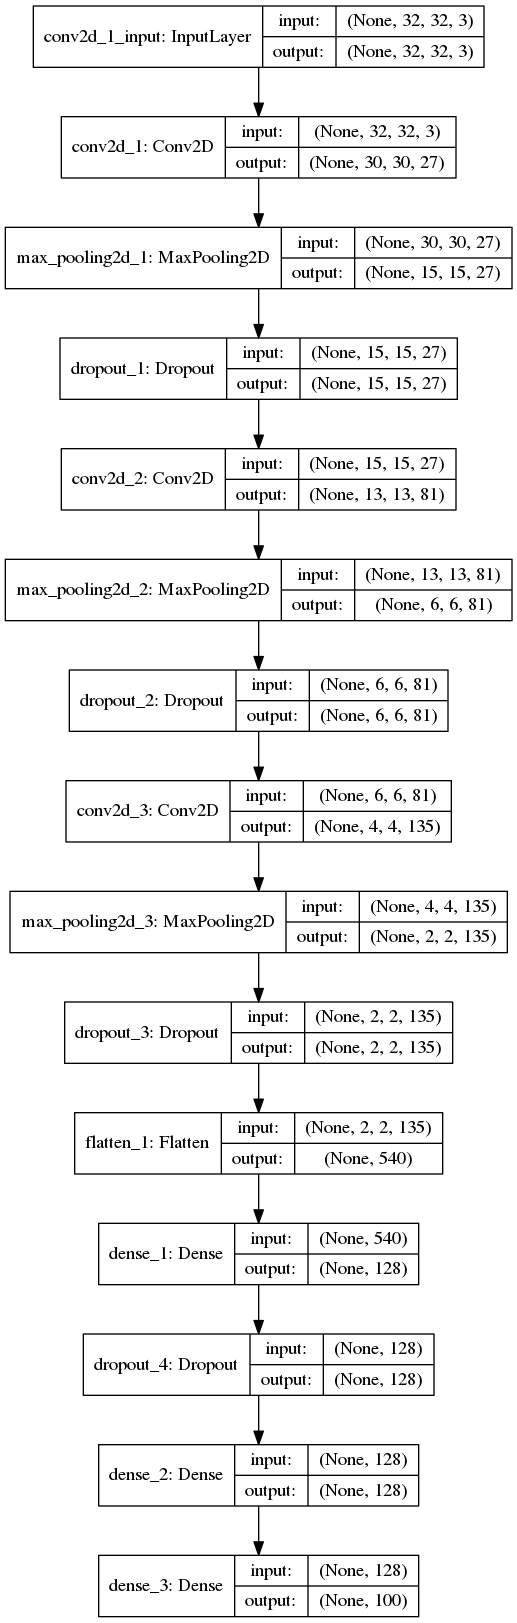
\includegraphics[width=0.45\textwidth]{dropout}
	\caption{Model with dropout.}
	\label{f:drop1}
\end{figure}

\end{document}
